\documentclass{chi-ext}
% Please be sure that you have the dependencies (i.e., additional LaTeX packages) to compile this example.
% See http://personales.upv.es/luileito/chiext/

\usepackage{tikz}
\usepackage{verbatim}
%\usepackage[active,tightpage]{preview}
%\PreviewEnvironment{tikzpicture}

\copyrightinfo{
  Copyright is held by the author/owner(s).\\
  \emph{MobileHCI 2014}, September 23-26 2014, Toronto, Canada.\\
  ACM 978-1-XXXX-XXXX-X/XX/XX.\\
}

\title{Simple Visual and Vibrotactile Patterning within Wearable Mobile Gaming Experiences}

\numberofauthors{5}
% Notice how author names are alternately typesetted to appear ordered in 2-column format;
% i.e., the first 4 authors on the first column and the other 4 authors on the second column.
% Actually, it's up to you to strictly adhere to this author notation.
\author{
  \alignauthor{
  	\textbf{Adam Tindale}\\
  	\affaddr{OCAD University}\\
  	\affaddr{Toronto, ON M5T 1W1 Canada}\\
  	\email{atindale@faculty.ocadu.ca}
  }\alignauthor{
  	\textbf{Jessica Peter}\\
  	\affaddr{OCAD University}\\
  	\affaddr{Toronto, ON M5T 1W1 Canada}\\
  	\email{jp11jg@student.ocadu.ca}
  } 
    \vfil
  \alignauthor{
  	\textbf{Michael Cumming}\\
  	\affaddr{OCAD University}\\
  	\affaddr{Toronto, ON M5T 1W1 Canada}\\
  	\email{mcumming@ocadu.ca}
  }\alignauthor{
  	\textbf{Sara Diamond}\\
  	\affaddr{OCAD University}\\
  	\affaddr{Toronto, ON M5T 1W1 Canada}\\
  	\email{sdiamond@ocadu.ca}
  }
    \vfil
    \alignauthor{
  	\textbf{Hudson Pridham}\\
  	\affaddr{OCAD University}\\
  	\affaddr{Toronto, ON M5T 1W1 Canada}\\
  	\email{hp12pk@student.ocadu.ca}
  } 
}

% Paper metadata (use plain text, for PDF inclusion and later re-using, if desired)
\def\plaintitle{Simple Visual and Vibrotactile Patterning within Transmedia Gaming Experiences}
\def\plainauthor{Adam Tindale}
\def\plainkeywords{pattern recognition, wearable devices, gaming, multi-sensory, vibrotactile}
\def\plaingeneralterms{Gaming, Patterns, Wearable}

\hypersetup{
  % Your metadata go here
  pdftitle={\plaintitle},
  pdfauthor={\plainauthor},  
  pdfkeywords={\plainkeywords},
  pdfsubject={\plaingeneralterms},
  % Quick access to color overriding:
  citecolor=black,
  linkcolor=blue,
  menucolor=black,
  urlcolor=blue,
}

\usepackage{graphicx}   % for EPS use the graphics package instead
\usepackage{balance}    % useful for balancing the last columns
\usepackage{bibspacing} % save vertical space in references
\usepackage{paralist}
\usetikzlibrary{shapes,arrows}

\begin{document}
\maketitle

\begin{abstract}
%Simple, wearable devices are a promising way of encouraging participation with those who consume, and contribute to, media. 

In this paper we describe a series of demo experiences focusing on the communication of information through low resolution vibrotactile and LED displays. The intended purpose for this exploration is to add simple visual and vibro-tactile patterning to wearable devices intended for children aged 8-12. These patterns add sensory interest to these devices and convey useful information about device dynamics and expected user interactions. 
\end{abstract}

\keywords{\plainkeywords}

\category{H.5.2}{Information interfaces and presentation (e.g., HCI)}{User Interfaces}. 

\terms{\plaingeneralterms}

% ===========================================================================
\section{Introduction}
% ===========================================================================

The research questions we address in this paper concern whether it is possible to create wearable gaming experiences that involve simple visual and vibrotactile patterns. Some  research questions of interest to us are:
\begin{inparaenum}[\itshape a\upshape)]
\item what types of pattern for wearable devices seem appropriate?
\item what functions can such patterns perform?
\item how can haptic actuators interact with buttons and lights?
\item is the best way to employ these patterns for the conveyance of information or for some other purpose?
\end{inparaenum}

What then is a simple pattern? I could be as simple a one dimensional (1D) line of LED lights. 

\subsection{Some examples of simple patterns}
\bigskip
\begin{figure}
  	\begin{center}
	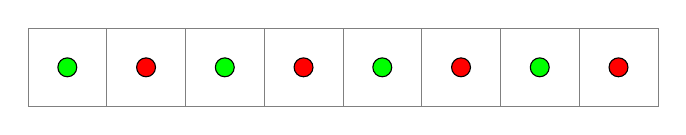
\begin{tikzpicture}
	%green LEDs
	\draw[step=1cm,gray,very thin] (0,0) grid (8,1);
	\filldraw[fill=green, draw=black] (0.5,0.5) circle (0.12cm);
	\filldraw[fill=green, draw=black] (2.5,0.5) circle (0.12cm);
	\filldraw[fill=green, draw=black] (4.5,0.5) circle (0.12cm);
	\filldraw[fill=green, draw=black] (6.5,0.5) circle (0.12cm);
	%red LEDs
	\filldraw[fill=red, draw=black] (1.5,0.5) circle (0.12cm);
	\filldraw[fill=red, draw=black] (3.5,0.5) circle (0.12cm);
	\filldraw[fill=red, draw=black] (5.5,0.5) circle (0.12cm);
	\filldraw[fill=red, draw=black] (7.5,0.5) circle (0.12cm);

	\end{tikzpicture}
  	\caption{1D grid of green and red LED lights.}
  	\label{fig:1D}
    	\end{center}
\end{figure}

The next step in complexity are simple 2D grids of LED lights, buttons and vibro-tactile actuators. A device with such inputs and outputs affords many types of interactions and notification possibilities:
\bigskip
\begin{figure}
  	\begin{center}
	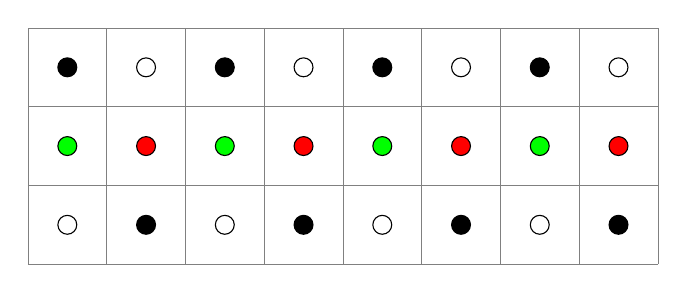
\begin{tikzpicture}
	%green LEDs
	\draw[step=1cm,gray,very thin] (0,0) grid (8,3);
	\filldraw[fill=green, draw=black] (0.5,1.5) circle (0.12cm);
	\filldraw[fill=green, draw=black] (2.5,1.5) circle (0.12cm);
	\filldraw[fill=green, draw=black] (4.5,1.5) circle (0.12cm);
	\filldraw[fill=green, draw=black] (6.5,1.5) circle (0.12cm);
	%red LEDs
	\filldraw[fill=red, draw=black] (1.5,1.5) circle (0.12cm);
	\filldraw[fill=red, draw=black] (3.5,1.5) circle (0.12cm);
	\filldraw[fill=red, draw=black] (5.5,1.5) circle (0.12cm);
	\filldraw[fill=red, draw=black] (7.5,1.5) circle (0.12cm);
	%topButtons
	\filldraw[fill=black, draw=black] (0.5,2.5) circle (0.12cm);
	\filldraw[fill=black, draw=black] (2.5,2.5) circle (0.12cm);
	\filldraw[fill=black, draw=black] (4.5,2.5) circle (0.12cm);
	\filldraw[fill=black, draw=black] (6.5,2.5) circle (0.12cm);
	%bottomButtons
	\filldraw[fill=black, draw=black] (1.5,0.5) circle (0.12cm);
	\filldraw[fill=black, draw=black] (3.5,0.5) circle (0.12cm);
	\filldraw[fill=black, draw=black] (5.5,0.5) circle (0.12cm);
	\filldraw[fill=black, draw=black] (7.5,0.5) circle (0.12cm);
	%topVibes
	\filldraw[fill=white, draw=black] (1.5,2.5) circle (0.12cm);
	\filldraw[fill=white, draw=black] (3.5,2.5) circle (0.12cm);
	\filldraw[fill=white, draw=black] (5.5,2.5) circle (0.12cm);
	\filldraw[fill=white, draw=black] (7.5,2.5) circle (0.12cm);
	%bottomVibes
	\filldraw[fill=white, draw=black] (0.5,0.5) circle (0.12cm);
	\filldraw[fill=white, draw=black] (2.5,0.5) circle (0.12cm);
	\filldraw[fill=white, draw=black] (4.5,0.5) circle (0.12cm);
	\filldraw[fill=white, draw=black] (6.5,0.5) circle (0.12cm);
	
	%\filldraw[fill=black, draw=black] (1.2,2.4) rectangle (0.4,2.6cm);

	\end{tikzpicture}
  	\caption{2D array of LED lights, buttons (black-filled circles) and vibrating motors (white-filled circles).}
  	\label{fig:1D}
    	\end{center}
\end{figure}

The basic components used on the devices we discuss here are buttons, LED lights and vibrating motors. These elements can be arranged in a variety of 1D, 2D, or 3D arrays. At its simplest, user interactions involves pressing a button. Buttons can be used to select a pattern, to play a game involving flashing lights such as 'Simon Says' or to acknowledge a signal provided by the lights and vibrating motors.  

The patterns involve some kind of order that is apparent either visually or tactilely. The patterns generated may involve movement and may have directionality. These patterns may be useful in the conveyance of some information, such as the state of a game, a device or the gamer. The pattern may also be a signalling device within a game device to inform the gamer about some situation within her gaming or external environment.

Wearable devices are often hooked up wirelessly to other machines or devices. For instance, gaming controllers provide users with the opportunity to expertly control a game experience. However, game controllers are purpose-driven devices that provide little utility when not connected to the game experience. While there have been many interesting uses of game controllers outside of game experiences, the controllers themselves rely on being attached to hardware in order to have any function. 

Therefore, wearable device could have functions independent of other devices. They could be self-sufficient in their functionality. The patterns they present to the user could have some value outside the context of a larger gaming environment. 

Using simple components such as buttons, lights and vibrating motors a a device will have certain affordances. This paper explores what those affordances are and what their potential application might be. 

\subsection{Some possible functions for simple patterns}
\begin{inparaenum}[\itshape a\upshape)]
\item they could create pleasing visual or tactile sensations for the user
\item they could notify wearers of something of interest in their proximity
\item they could provide an identity for the wearer with light and vibratory patterns becoming a type of personal signature
\item and, they could provide a wearable 'authoring environment' for these types of decorative and informational functions. 
\end{inparaenum}

Interactions with such a device could be very simple, such that they convey information in a way that presents few cognitive demands on the user and which the user would tend to find enjoyable and engaging even if they were not participating in a mobile game. 

Our demo experiences focus on an attempt to make the interactions very simple, such that they convey information in a way that presents few cognitive demands on the user and which the user would tend to find enjoyable and engaging, even if they were not participating in a mobile game. 

%If well done they engage viewers and can build interesting, emergent social cohorts. They have the potential of explaining and making connections between complex concepts in a fluid and graceful way. However, because of this fluidity of structure they demand a high level of skill in their artistic conception and organization. 

%The basic device use cases that might inform the gamer during gameplay, which also could apply to a viewer navigating through a narrative, are: 
%\begin{inparaenum}[\itshape a\upshape)]
%  \item what is my current position or state within the game?
%  \item do I need to make any decisions or choices in order to proceed with the game?
%  \item is anything else happening in the game of which I should be aware? and,
%  \item what comes next in the game? 
%\end{inparaenum}

%For the social and collection aspects of a game like Time Tremors we have identified several important use cases: 
%\begin{inparaenum}[\itshape a\upshape)]
%\item detect other band wearers (wirelessly) who happen to be in the vicinity
%\item give something of value to another wearer, 
%\item exchange something of value with another wearer, and
%\item give the wearer some indication of the game mode the wearer is in.
%\end{inparaenum}

Our demo experiences focus on an attempt to make the interactions very simple, such that they convey information in a way that presents few cognitive demands on the user and which the user would tend to find enjoyable and engaging.

%Our goal is to create integrated user experiences that are simple and enjoyable. Our goal is despite how complex the game mechanics might be the device and how to use it remain relatively simple and straightforward.  

Our demo experiences focus on an attempt to make the interactions very simple, such that they convey information in a way that presents few cognitive demands on the user and which the user would tend to find enjoyable and engaging, even if they were not participating in a mobile game. 

% ======================================================================
\section{Related Work}
% ======================================================================

Ruspini provides a useful introduction to the concepts and history of haptics, the basics of haptic psychophysics and haptic devices past and present \cite{ruspini1999haptics}.

Bronner notes that a sense of touch is basic to human processes of testing, expressing reality and meaning. Often people must both see with their own eyes as well as touch with their own hands to believe in a phenomenon\cite{bronner1982haptic}. He also notes that people surround themselves with particular objects to reinforce their own feelings and identities. 

MacLean \cite{maclean2009putting} discusses the potential benefits of haptic feedback as an ambient notification system. Unlike visual information, which can be obtrusive while completing a task, or sound, which can be obnoxious in a public environment, haptic feedback is usually experienced only by the user and does not directly interfere with the task at hand. 

In Profita (2013) \cite{profita2013don} researchers reveal the results of studies completed in the United States and South Korea on the social acceptability of interacting with on-body controllers in which participants  ranked factors such as ?awkwardness? and ?coolness? of the exhibited interactions as actors performed them. This article is helpful for providing insight on social acceptability of wearable positioning as it relates to gender and culture.

Oliveira and Maciel propose a network of haptic actuators that use a set of patterns to express elements of an environment that has obstacles and free paths and demonstrates the use of a haptic language that helps users navigate and consists of vibrotactile signs to complement or replace their vision. \cite{Jesus-Oliveira:2013aa}

De Jesus Oliveira and Maciel \cite{Jesus-Oliveira:2013aa} present research towards building a hand-mounted array of haptic actuators intended to help the wearer perform a variety of tasks including orientation. They propose that the actuators could be connected to environment-aware sensors so that the actuators would vibrate in a set pattern to alert the wearer of an obstacle (or help instruct them to perform a certain task). Such haptic systems could help visually impaired users navigate. They would also enable fully sighted users to perform certain tasks without being distracted by personal technologies (i.e. using a smartphone to check a map).


% ======================================================================
\section{Prototypes and Case Studies}
% ======================================================================
\subsection{Simon Says Wristband}
Description: this is a wearable version of the traditional \emph{Simon Says} game mounted into a velcro and felt wristband. Unlike the rubber bands with their aggressive punk aesthetic this wristband is relatively sleek and wearable. It is sewn onto a flexible felt band. Conductive thread connects components, which aids wearability. The game is controlled by four push buttons, each with a corresponding LED light. This forms a 2x2 button and light matrix. The LEDs flash in a random pattern to begin a game session. A single vibration motor signals the beginning of a new game. To play the game the wearer repeats the pattern as flashed by the LEDs by pressing the buttons directly adjacent to each LED. The button and light array affords simple gaming possibilities. The components are low profile and are integrated into a device that is lightweight and comfortable to wear. 

This wristband's components are:
\begin{inparaenum}[\itshape a\upshape)]
\item Felt wristband and Velcro closer
\item Lilypad Arduino
\item Push buttons
\item LEDS (red, blue, yellow, green)
\item Vibration Motor
\item Conductive thread
\item Power supply
\end{inparaenum}

\begin{figure}
  \begin{center}
  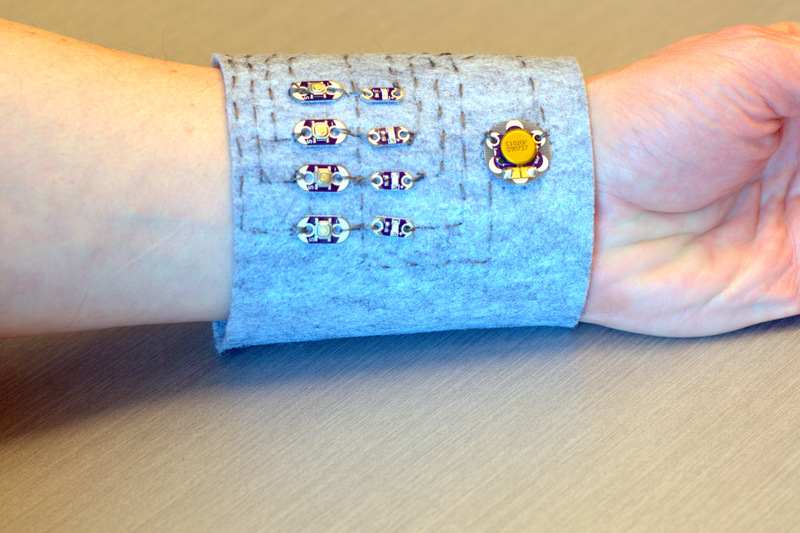
\includegraphics[width=\columnwidth]{images/P1130375.jpg}
  \caption{A wearable version of the traditional Simon Says game. The LEDs flash in a random pattern. The wearer must repeat the pattern flashed by the LEDs by pressing the buttons directly adjacent to each LED.}
  \label{fig:simonSays}
  \end{center}  
\end{figure}

\subsection{Screen-based Wrist Wearable}
This prototype is as yet, not wearable but has a compact OLED screen with a pixel  resolution of 128x128. The intention for this device was to support interactions with a collections and task-based transmedia game called Time Tremors. The screen displays several items of interest for simple task-based games: name of task, efficiency at completing task, time spent on task and visualization of task.

Currently, compact, relatively high resolution screens (for instance, in pixel resolution of 128x128, or 96x96) are compact, inexpensive and provide clear images, which enables high-density information display similar to that found on smartphone and tablet displays, yet in a very compact form factor. This is in contrast to other devices shown here that have very low resolution input and output arrays. High density visual displays requires different types of interactions compared to very low resolution arrays and require operating software quite different from that which low resolution input and output arrays require.

This prototype's components are:
\begin{inparaenum}[\itshape a\upshape)]
\item 2200 mAh LiPo battery
\item 128 x 128 pixel OLED display
\item 5V step-up for LiPo battery
\end{inparaenum}

\begin{figure}
  \begin{center}
  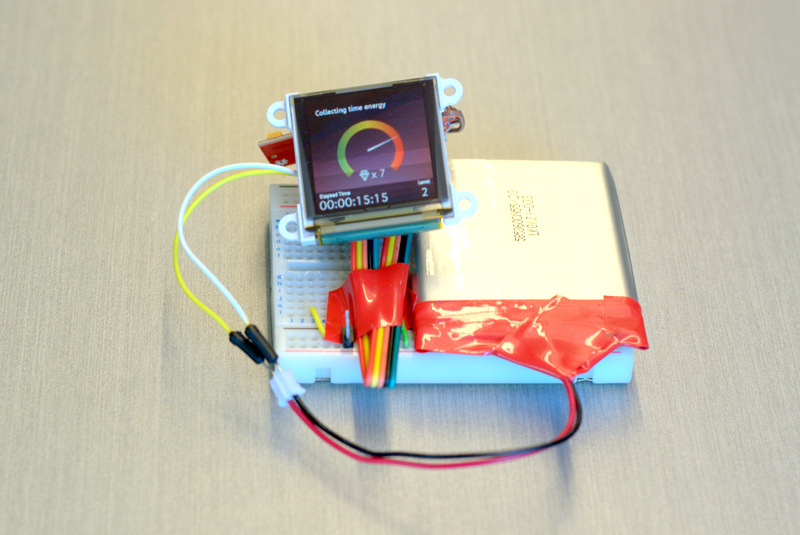
\includegraphics[width=\columnwidth]{images/P1130382.jpg}
  \caption{A prototype for a wearable that has a compact, yet high resolution OLED screen.}
  \label{fig:oledscreen}
  \end{center}  
\end{figure}

\subsection{Rubber vibration band version 1}
This wrist band with a thick rubber band has vibrating motors and LED lights. Vibrating motors and lights are arranged linearly with motors alternating with lights. It is connected to and controlled by an Arduino Mega board. The activation pattern of the lights and vibrators is linear and sequential; that is, they activate each in sequence to the end of the line and then repeat from the beginning. This sequential activation gives the band a simple haptic rhythm. Other types of haptic patterns are conceivable, such as rhythmic pulses, flashes and sequences with more complex rhythms. 

The device is very thick and can?t be worn (some components come out the back of the device). It is also hard-wired to an Arduino board, which also prevents wearability. The device has no input buttons or other input devices. The device makes a repetitive rhythmic sound by nature of its simple looping activation pattern. Other activation patterns could be programmed using the same components. These rhythms can be enjoyed in their own right as simple proto-musical patterns. Rhythmic, haptic patterns could also convey certain types of information, such as game mode, beginning of new sessions, ends of a session, arrival into a new playing zone, etc. 

This wristband's components include	:
\begin{inparaenum}[\itshape a\upshape)]
\item 16mm x 6mm mobile phone vibrators (Panasonic)
\item LED lights (red/green)
\item rubber band (conveyor belt material)
\item Arduino Mega 2560 controller board, w/ wired connectors
\end{inparaenum}

\begin{figure}
  \begin{center}
  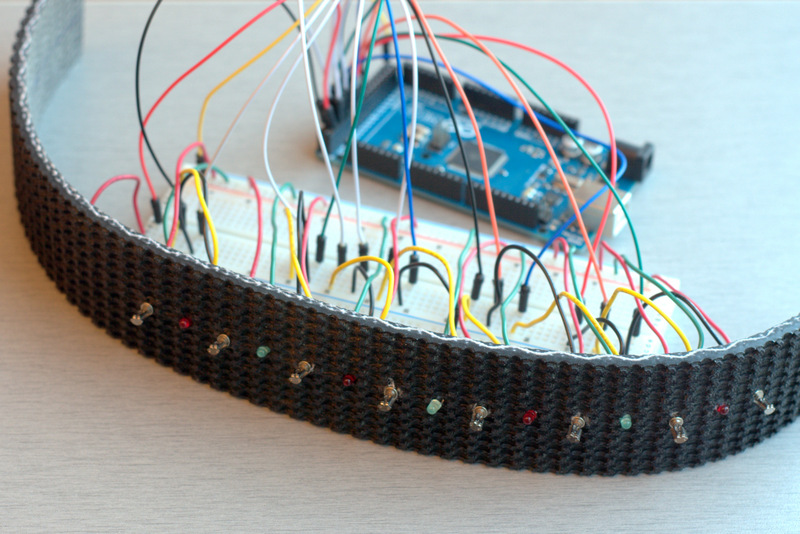
\includegraphics[width=\columnwidth]{images/P1130394.jpg}
  \caption{A prototype for a wearable that has a simple 1D array of LED light and vibrating motors.}
  \label{fig:marginparsample}
  \end{center}  
\end{figure}

\subsection{Rubber vibration band version 2}
This band is similar to the first band nut instead of a linear pattern, there is 3x8 array of buttons, lights and vibrating motors. Each row of this array has one button, one light and one vibrator. The buttons are programmed to activate the other two components in their row, to activate patterns across the whole array, (such as all the lights flashing at once, all vibrators at once, all red lights in sequence, all top vibrators in sequence, etc.), and to create interactive buttons games like \emph{Simon Says}.

This version like the first is not possible to wear in its current configuration due to the connection to its controlling Arduino board and thickness of its components. It presents a certain \emph{punk} aesthetic due to the thickness of the rubber band and the aggressiveness of the rotating vibrating motors. For some users, this might be an attractive feature. The 3x8 matrix starts to afford some interesting possibilities for user interaction. Modal play becomes possible since there are so many types of signals possible. For instance, all red lights could flash to indicate entering into a certain game mode. Therefore, some plausible use cases for the wristband could involve a simple wearable game involving button pushing; it could become the target device for authoring of light and vibration patterns, or it could be signalling device (if connected to wireless components) when in proximity to people or objects.

This wristband's components include:
\begin{inparaenum}[\itshape a\upshape)]
\item 16mm x 6mm mobile phone vibrators (Panasonic)
\item LED lights (red/green)
\item rubber band (conveyor belt material)
\item Arduino Mega 2560 controller board, w/ wired connectors
\item Push buttons (push on / norm off); Each individual component has its own digital pin on the Arduino board (3x8 = 24 pins in total).
\end{inparaenum}

\begin{figure}
  \begin{center}
  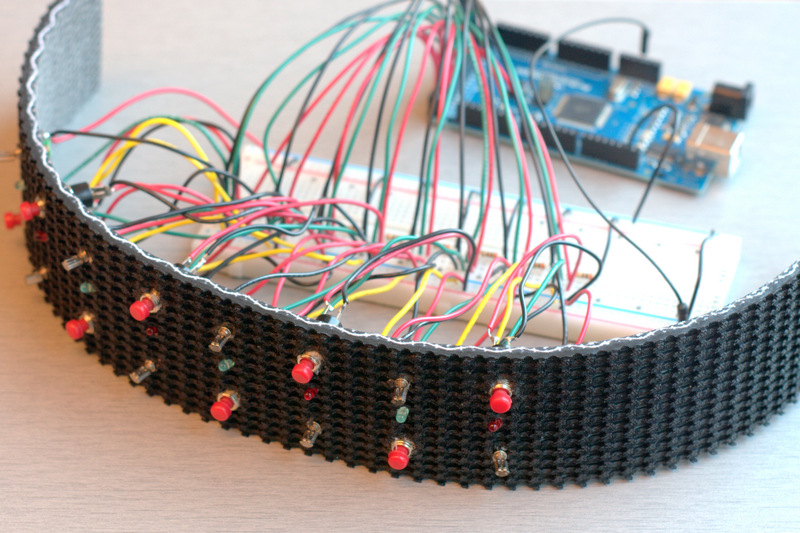
\includegraphics[width=\columnwidth]{images/P1130396.jpg}
  \caption{A prototype for a wearable that has a 3x8 array of buttons, LED lights and vibrating motors.}
  \label{fig:marginparsample}
  \end{center}  
\end{figure}

\subsection{Patterns}
The prototypes consist of simple arrays of vibrating motors and LED lights. Later prototypes add buttons to these components. What patterns can be created when using these components? The simplest are non-directional ones, such as flashing patterns [all on, then all off]. Other simulate movement using 1D and 2D transformations.

\subsection{Types of Patterns}
We have found that even the simplest patterns can convey interesting sensations with informational potential. A simple one-dimensional row of LED lights can flash in several different ways: \begin{inparaenum}[\itshape a\upshape)]
\item it can flash all its LEDs at once
\item it can flash in a sequential, directional pattern. 
\item it can vary the intensity of the LEDs in a pulsating pattern
\item it can illuminate only the red or the green LEDs, and
\item it can flash its lights in a random pattern. 
\end{inparaenum}

\begin{inparaenum}[\itshape a\upshape)]
\item flashing, non-directional ones in which all the lights or all the vibe motors activate at the same time. These might be useful, for instance, when the gamer has achieved a new level in a game;
\item flashing, directional ones which there is a sequential activation such that they appear to point in a specific direction. These could be used when the gamer detects another player in the vicinity and the device shows the direction where the other player is located;
\item flashing, expanding ones where a pattern is generated from a 'point of impact' and expands outwards in 2D, similar to what you might find in the 'Game of Life'
\end{inparaenum}

\subsection{Functions for Patterns}
TBD

\subsection{Development of prototypes}
Prototypes began as the simplest and least refined expression of a wearable or functional haptic device. The first prototype has simple linear arrangement of LED light and mobile phone type vibrating motors. When the connected to an Arduino micro-controller this band emits a rhythmic and visual sequential pattern that could conceivably could be used to notify band wearers of others in their vicinity. Although this band was perhaps the most simplistic band possible, it could in fact be functional in some minimal sense for a transmedia gaming experience. Also, such a minimal band would be inexpensive to manufacture and simple to program. 

Prototypes began as the simplest and least refined expression of a wearable or functional haptic device. The first prototype has simple linear arrangement of LED light and mobile phone type vibrating motors. When the connected to an Arduino micro-controller this band emits a rhythmic and visual sequential pattern that could conceivably could be used to notify band wearers of others in their vicinity. Although this band was perhaps the most simplistic band possible, it could in fact be functional in some minimal sense for a gaming experience. 

\marginpar{
\begin{figure}
  \begin{center}
  \includegraphics[width=\marginparwidth]{images/P1130386.jpg}
  \caption{A simple prototype that features visual and vibrotactile sensory outputs.}
  \label{fig:rubberVibeBand01}
  \end{center}  
\end{figure}
}

\section{Discussion and Conclusions}
This paper has demonstrated a number of interfaces that provide wrist based vibrotactile displays. Our work has shown that providing a vibrotactile array instead of a simple vibration motor provides user with a many more pathways of receiving and perceiving information.

\subsection{Wearability and Testing}
These kind of devices at the prototype stage are far from being wearable. They are typically connected to an Arduino board and have bulky components and wired connections that interfere with basic wearability. This makes testing of such devices in a natural context difficult or impossible. A question that arises is how to decide, in an evidence-based manner, which devices to develop further such that they become miniaturized and wearable. 

There are two types of patterns involved: there are the simple grids of the components themselves, and then there are the patterns which can generated using these simple components. When lights and vibrating motors can actuate in a dynamic way, then the dynamics that can be designed, such as flashes, waves and very low resolution visual images, can produce very interesting effects. 


%\section{Future Work}
%Wearable devices and associated technologies for developing is developing at a rapid pace.
%Miniaturization, bearability and functionality is obviously a primary concern of such devices. 

\section{Acknowledgements}
%We thank the valuable input from Patrick Crowe and all those at Xenophile Media Inc. who have great expertise in crafting transmedia narratives; Dr. Rachel Zuannon from the Graduate Design Program at Anhembi Morumbi University, Sao Paulo, Brazil.; the professors, students and staff within OCAD University's Digital Futures Initiative (DFI) for their valuable input and helpful comments. The following students within the DFI program worked on this project over many months: Hudson Pridham, Ryan Maksymic, Jessica Peter and Boris Kourtoukov. We thank Dr. Steve Szigeti for his contributions to this project and we especially thank Dr. Sara Diamond, President of OCAD University for her guidance and support.

We would like to thank Ryan Maksymic, Boris Kourtoukov, and Steve Szigeti for their help in the development of this project. This work is generously supported by grants from the Natural Sciences and Engineering Research Council of Canada (NSERC), International Science and Technology Partnerships Canada.

\balance
\bibliographystyle{acm-sigchi}
\bibliography{MGDSPET}

\end{document}
